\chapter{Results}

\section{Empirical Evaluations}


\begin{shaded}
  Describe results
  \end{shaded}

The most interesting result from the experiements can be seen in the plot of the relative error for 100 000 highscore updates in figure \ref{fig:relerror}.

The relative error seems to -- quite naturally -- take off exponentially while the improved algorithm seems to produce consistent results after all updates.

\begin{figure}[h!]
  \centering
  \caption{Relative error for 100 000 highscore updates. Red line is the old algorithm, green line is the algorithm with dynamic bucket-table}
  \label{fig:relerror}
  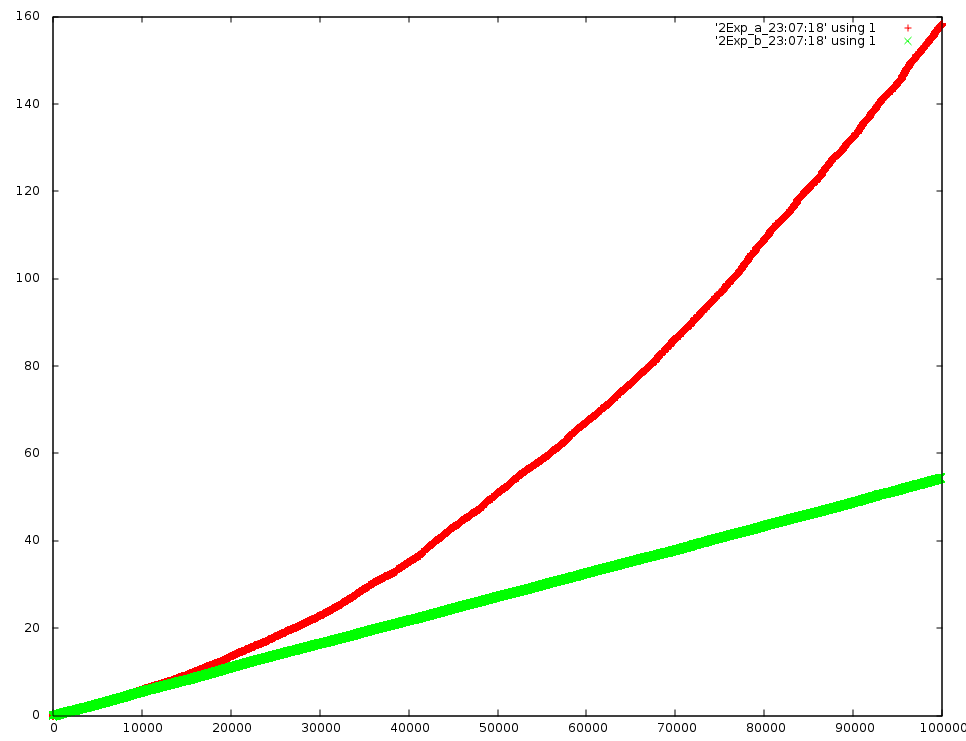
\includegraphics[width=10cm]{img/relative}
\end{figure}




